\chapter{Compound Interest}

When you loan money to someone, you typically charge them some sort of
interest. The most common loan of this sort is what the bank calls a
``savings account''.  Any money you put in the account is loaned to
the bank. The bank then lends it to someone else, who pays interest to
the bank. The bank gives some of that interest to you.
% Diagram needed
However, what if you leave the interest in your account? And you start
making \textit{interest on the interest}? This is known as
\textit{compound interest}.\index{compound interest}

\section{An example with annual interest payments}

Let's say that you put \$1000 in a savings account that pays 6\%
interest every year. How much money would you have after 12 years?
Let's make a spreadsheet.

\includegraphics[width=0.4\textwidth]{StartInterest.png}

Create a new spreadsheet and edit the cells to look like this.  All
the cells in rows 1 - 4 are just values: just type in what you
see.

The fifth row is all formulas:

\begin{tabular}{c | c | c}
  After year & Interest & Balance \\
  \hline 
  = A4 + 1 & = B\$1 * C4 & = C4 + B5 \\
\end{tabular}

The interest rate field should be formatted as a percentage. One thing
to know when dealing with percentages in the spreadsheet: If the field
says ``600\%'', its value is 6. 

The cells in the Interest and Balance column should be formatted as currency.

You are about to make several copies of the cells in the fifth row,
so make sure they look right.

Click on A5 and shift-click on C5 to select all three cells. Drag the
lower-right corner down to fill the rows 6 - 15.

\includegraphics[width=0.5\textwidth]{CopiedCellsInterest.png}

Look at the numbers.  The first interest payment is \$60, but the last
is \$113.90. Your balance has more than doubled!

\section{Exponential Growth}

We figured this out numerically by repeatedly multiplying the balance
by the interest rate. What if you wanted to know what the balance
would be $n$ years after investing $P_0$ dollars with an annual interest
rate of $r$? (Note that $r$ in our example would be 0.06, not 6.0.)

Each year, the balance is multiplied by $1 + r$, so after one year,
$P_0$ would become $P_0 \times (1 + r)$.  The next year you would multiply
this number by $(1 + r)$ again: $P_0 \times (1 + r) \times (1 + r)$. The
next year? $P_0 \times (1 + r) \times (1 + r) \times (1 + r)$ See the
pattern? $P_n$ is this balance after $n$ years, then
\begin{equation}
  P_n = P_0 (1+r)^n
  \label{eq:compound}
\end{equation}

\ref{eq:compound} is referred to as the standard \newterm{compound interest formula}. 
Because $n$ is an exponent, we call this \textit{exponential growth}.
There are few things as terrifying to a scientist as
the phrase ``The population is undergoing exponential growth''.\index{exponential growth}

If the principal is not compounded annually, we can modify the equation to account for that by changing $n$.

$$n = m t$$

Where $t$ is the frequency of the compounding, called the period: (1: annually, 12: monthly, 52: weekly, 365: daily), and $m$ is the number of periods. 
This equation becomes
$$P_n = P_0 (1+\frac{r}{n})^{nt}$$
We will see these two terms pop up in other areas of the curriculum like circular motion and waves.
% Diagram/ Explain

\section{Sensitivity to interest rate}

For most people, the first surprising thing about compound interest is
how quickly your money grows after a few years.  The second thing that
is surprising is how much difference a small change in the percentage
rate makes.

Let's add another set of columns that shows what happens to your money
if you convince the bank to pay you 8\% instead of 6\%.

Copy everything from columns B and C:

\includegraphics[width=0.6\textwidth]{CopyForSecondInterest.png}

Now edit the second interest rate to be 8\%:

\includegraphics[width=0.6\textwidth]{AtBiggerInterestRate.png}

\section{Continuous Compound Interest}
Let's say, hypothetically, that we compound interest on a given balance for an \emph{indefinite} amount of time. Then, we take the formula $$P_n = P_0 (1+\frac{r}{n})^{nt}$$

What if we divide our time period into infinite chunks? This would mean splitting our $n$ into much smaller pieces. We can use calculus notation to find the limit of this:
\begin{equation*}
  \lim_{n \rightarrow \infty} P_0 (1+\tfrac{r}{n})^{nt}
\end{equation*}
we can create a variable $x=\frac{n}{r}$. We do this so that we eliminate some other dummy variables. Now we have
\begin{equation*}
  \lim_{n \rightarrow \infty} P_0 (1+\tfrac{1}{x})^{xrt}
\end{equation*}
as we can eliminate $n$ with $n=xr$.

Now we can isolate parts of our compound interest equation into the limit, and extract variables out.

\begin{equation*}
  P_0 \left(\lim_{n \rightarrow \infty} (1+\tfrac{1}{x})^{x}\right)^{rt}
\end{equation*}


Fun math fact: $\lim_{n \rightarrow \infty} (1+\tfrac{1}{x})^{x}$ is equal to the mathematical constant $e$. We are going to dive into this in the \emph{logs} chapter! For now, just understand that it is a constant in mathematics that describes many growth or decay values. With that, we can simplify the equation as the continuous compound interest equation (\ref{eq:continuous_compound})
\begin{equation}\label{eq:continuous_compound}
  P_0e^{rt}
\end{equation}

\section{Practice Exercises}

\begin{Exercise}[label=compoundinterest1]
You deposit \$1500 into a savings account that pays an annual interest
rate of 5\%, compounded annually. What is the balance after 8 years?

Note: you can also use excel or google sheets built in function \texttt{=FV()}.
\end{Exercise}

\begin{Answer}[ref=compoundinterest1]
Using \ref{eq:compound} with $P_0 = 1500$, $r = 0.05$, and $n = 8$:
$$P_8 = 1500 (1+0.05)^8 = 1500 (1.05)^8 \approx \$2216.18$$

Alternatively, in Sheets/Excel, we can use \texttt{=FV(0.05, 8, 0, -1500)} to say that we want the \newterm{future value} of 1500 deposited (hence, negative), after 8 years compounded once per year.
\end{Answer}

\begin{Exercise}[label=compoundinterest2]
A bank offers two savings accounts, both with a stated annual interest
rate of 6\%. Account A compounds monthly ($t = 12$) and Account B
compounds daily ($t = 365$). If you deposit \$3000 into each account,
which account has the higher balance after 5 years, and by how much?

Create two columns in Excel/Sheets showing the balance after each year
for each account, using \$3000 as the principal. Start with year 0 for the
initial deposit, then fill in years 1 through 5 using the compound
interest formula for monthly and daily compounding.
\end{Exercise}

\begin{Answer}[ref=compoundinterest2]
Using $P_n = P_0 (1+\frac{r}{n})^{nt}$ with $P_0 = 3000$, $r = 0.06$, and $n = 5$ years:

Account A (monthly, $t=12$):
$$P = 3000 \left(1+\frac{0.06}{12}\right)^{12 \times 5} \approx \$4046.55$$

Account B (daily, $t=365$):
$$P = 3000 \left(1+\frac{0.06}{365}\right)^{365 \times 5} \approx \$4049.48$$

\begin{figure}[H]
    \centering
    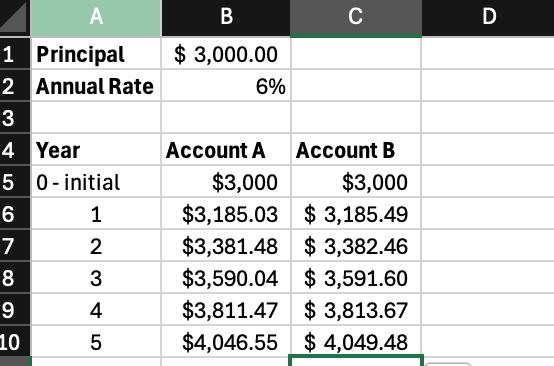
\includegraphics[width=0.8\textwidth]{exercise2sheet.png}
\end{figure}

Account B has the higher balance, by about \$2.93. This makes sense:
the more frequently interest is compounded, the closer the balance
gets to the continuous compounding limit, $P_0 e^{rt}$.
\end{Answer}
